\documentclass[11pt,a4paper]{article}
\usepackage[margin=2.2cm]{geometry}
\usepackage{graphicx,booktabs,amsmath,amssymb,xcolor,hyperref,caption,enumitem}
\hypersetup{colorlinks,linkcolor=blue!50!black,urlcolor=blue!50!black}
\setlist{itemsep=2pt,topsep=4pt}
\newcommand{\eps}{\varepsilon}
\newcommand{\epsd}{\dot{\varepsilon}}
\newcommand{\tauII}{\tau_\mathrm{II}}

\title{Interface-cell averaging schemes in StagFDTools:\\ shear apparatus and Viagra benchmarks}
\author{StagFDTools, branch \texttt{test-voigt-reuss}}
\date{15 November 2026}

\begin{document}
\maketitle

\begin{abstract}
Seven ways of evaluating the visco-elasto-plastic rheology in cells that contain more than one phase are compared after two bug fixes, a corrected plastic strain and implicit strain hardening. The tests are the shear apparatus at medium resolution ($140\times500$, gouge at $\theta=40^\circ$) and the elastic Viagra cantilever. Iso-strain-rate (Voigt) averaging on the grid gives the cleanest stress field and the most robust convergence, at the cost of the legacy scheme. It is the recommended default. Marker-based averaging gives no measurable gain for 1.4--2.1 times the wall time. Iso-stress averaging on markers does not converge in the apparatus.
\end{abstract}

\section{Schemes}

A cell (centroid or vertex) containing phases $i$ with volume fractions $\phi_i$ needs one stress $\boldsymbol\tau$ and one tangent $\mathbf D = \partial\boldsymbol\tau/\partial\epsd$ for the Stokes solver. The schemes differ in how the cell strain rate $\epsd$ is partitioned among the phases and where the averaging is done.

\begin{description}
\item[0 legacy (\texttt{default})] Each phase sees the cell strain rate and a shared old stress $\boldsymbol\tau^0$. The stresses are averaged with the phase fractions, and a harmonic grid shear modulus is used for all phases.
\item[1 iso-strain, grid (\texttt{voigt})] $\epsd_i=\epsd$, with an old stress and old pressure per phase ($\boldsymbol\tau^0_i$, $P^0_i$) carried by the markers. The cell stress is $\sum_i\phi_i\boldsymbol\tau_i$. This is exact for phases in parallel.
\item[2 iso-strain, markers (\texttt{markers})] Same rule, but the rheology is evaluated on every marker with the control-volume strain rate and then averaged. The plastic strain is integrated on each marker.
\item[3 iso-stress, grid (\texttt{reuss})] $\boldsymbol\tau_i=\boldsymbol\tau$ and $\sum_i\phi_i\epsd_i=\epsd$, solved by an inner Newton iteration on the per-phase $\epsd_{\mathrm{II},i}$. This is exact for phases in series.
\item[4 iso-stress, markers (\texttt{markers\_stress})] Tensor Reuss partition over the markers of a control volume.
\item[5 iso-work, grid (\texttt{isowork})] $\epsd_i=a_i\epsd$ with $\sum_i\phi_i a_i=1$. The multipliers $a_i$ are chosen so that the work increment $(\boldsymbol\tau_i(a)-\boldsymbol\tau_i(0)):a_i\epsd$ is the same in every phase. This lies between Voigt and Reuss.
\item[6 iso-work, markers (\texttt{markers\_work})] Same rule over the markers.
\end{description}

\paragraph{Common to all runs.} The accumulated plastic strain is $\eps_p=\int\epsd_\mathrm{II}^{pl}\,dt$ with $\epsd^{pl}_\mathrm{II}=\epsd_\mathrm{II}(1-\tau_\mathrm{II}/\tau^{ve}_\mathrm{II})$. It is the invariant of the plastic deviatoric strain rate; the older $\int\dot\lambda\,dt$ was twice as large on the Drucker--Prager branch. The plastic strain is advected with the markers: per phase for the grid schemes, and per marker for the marker schemes. Strain hardening $C=C_0+\Delta C\tanh(\eps_p/\eps_h)$ is implicit: the end-of-step $\eps_p$ is found by a bracketed scalar solve around the return mapping. The friction angle of the gouge is the measured $\phi=34^\circ$.

\section{Bugs fixed before the comparison}

All results obtained earlier with the apparatus were affected by these bugs; the first two are also present on \texttt{main}.

\begin{enumerate}
\item \textbf{Unfilled ghost cells.} The ghost cells of the new centroid fields ($P$, $\tau_{xx}$, $\tau_{yy}$, $\epsd$, $\eta$, per-phase stresses and pressures, $\epsd^{pl}$) were never filled, while the old fields had zero-gradient ghosts. Markers within half a cell of a boundary therefore received wrong increments (0 minus the old value). With per-phase pressure, about 44\% of the pressure change was lost at the walls each step. Fix: \texttt{fill\_centroid\_ghosts!} (periodic-aware), called after each solve.
\item \textbf{Pressure overwritten in the legacy phase loop.} In mixed cells the dilatancy correction of one phase became the input of the next, which gave 32--35\% too much dilatancy. Fix: a separate pressure per phase.
\item \textbf{Allocation in the continuity assembly.} \texttt{ad\_partial\_gradients} built its argument tuple with a runtime index. Julia could not infer the tuple type, so the assembly allocated in every cell (33.6\,MB per Jacobian at $70\times250$). Fix: the code is now unrolled at compile time. This also benefits \texttt{StokesDeformed}, \texttt{ThermoMechanics}, \texttt{StokesFSG} and the two-phase solvers.
\end{enumerate}

\paragraph{Dilatancy check.} In a confined free-slip box with two identical phases arranged as a checkerboard, the pressure must rise as $\dot P = K\sin\psi\,\dot\lambda$. After the fixes, the legacy scheme and iso-strain (with per-phase or shared pressure) all give a ratio $\dot P/(K\sin\psi\,\dot\lambda)=1.0000$ for $\psi=15^\circ$ and $34^\circ$. $P$ stays constant for $\psi=0$.

\section{Allocations}

Each kernel was timed with \texttt{@allocated} on a real apparatus state with the gouge yielding, at two resolutions. Table~\ref{tab:alloc} shows the same values at $35\times125$ and $70\times250$ for every scheme. What remains is the fixed cost of the threaded loops: an empty \texttt{Threads.@threads} loop costs 2.2--2.5\,kB with 6 threads and 0.4\,kB with 1. Neither the rheology (including the inner Newton iterations of iso-stress and iso-work, and implicit hardening) nor the assembly allocates per cell. Test: \texttt{ShearApparatus/\_alloc\_test/alloc\_test.jl}.

\begin{table}[h]\centering\small
\caption{Bytes per call, the same at both resolutions.}\label{tab:alloc}
\resizebox{\textwidth}{!}{\begin{tabular}{lrr}
\toprule
kernel & 6 threads & 1 thread\\
\midrule
\texttt{TangentOperator!} (rheology + AD tangent), grid schemes & 16\,160 & 2\,784\\
\texttt{TangentOperator!}, marker schemes & 33\,248 & 5\,632\\
\texttt{ResidualContinuity2D!} / \texttt{Momentum2D\_x!} / \texttt{\_y!} & 5\,296 / 6\,064 / 6\,448 & 928 / 1\,056 / 1\,120\\
Jacobian or preconditioner assembly (before the fix: 33.6\,MB at $70\times250$) & 43\,936 & 17\,312\\
\bottomrule
\end{tabular}}
\end{table}

\section{Shear apparatus}

\paragraph{Fit and resolution.} With scheme~1, the gouge parameters $C=1.25+2.8\tanh(\eps_p/0.5)$\,MPa, $\phi=34^\circ$, $\psi=11.7^\circ$ fit the lab apparent friction at $\theta=30,40,50^\circ$. The rms misfit is 0.0054/0.0044/0.0079 at LR and 0.0060/0.0075/0.0086 at MR (Fig.~\ref{fig:res}). The final friction differs by at most 0.008 between LR and MR.

\begin{figure}[h]\centering
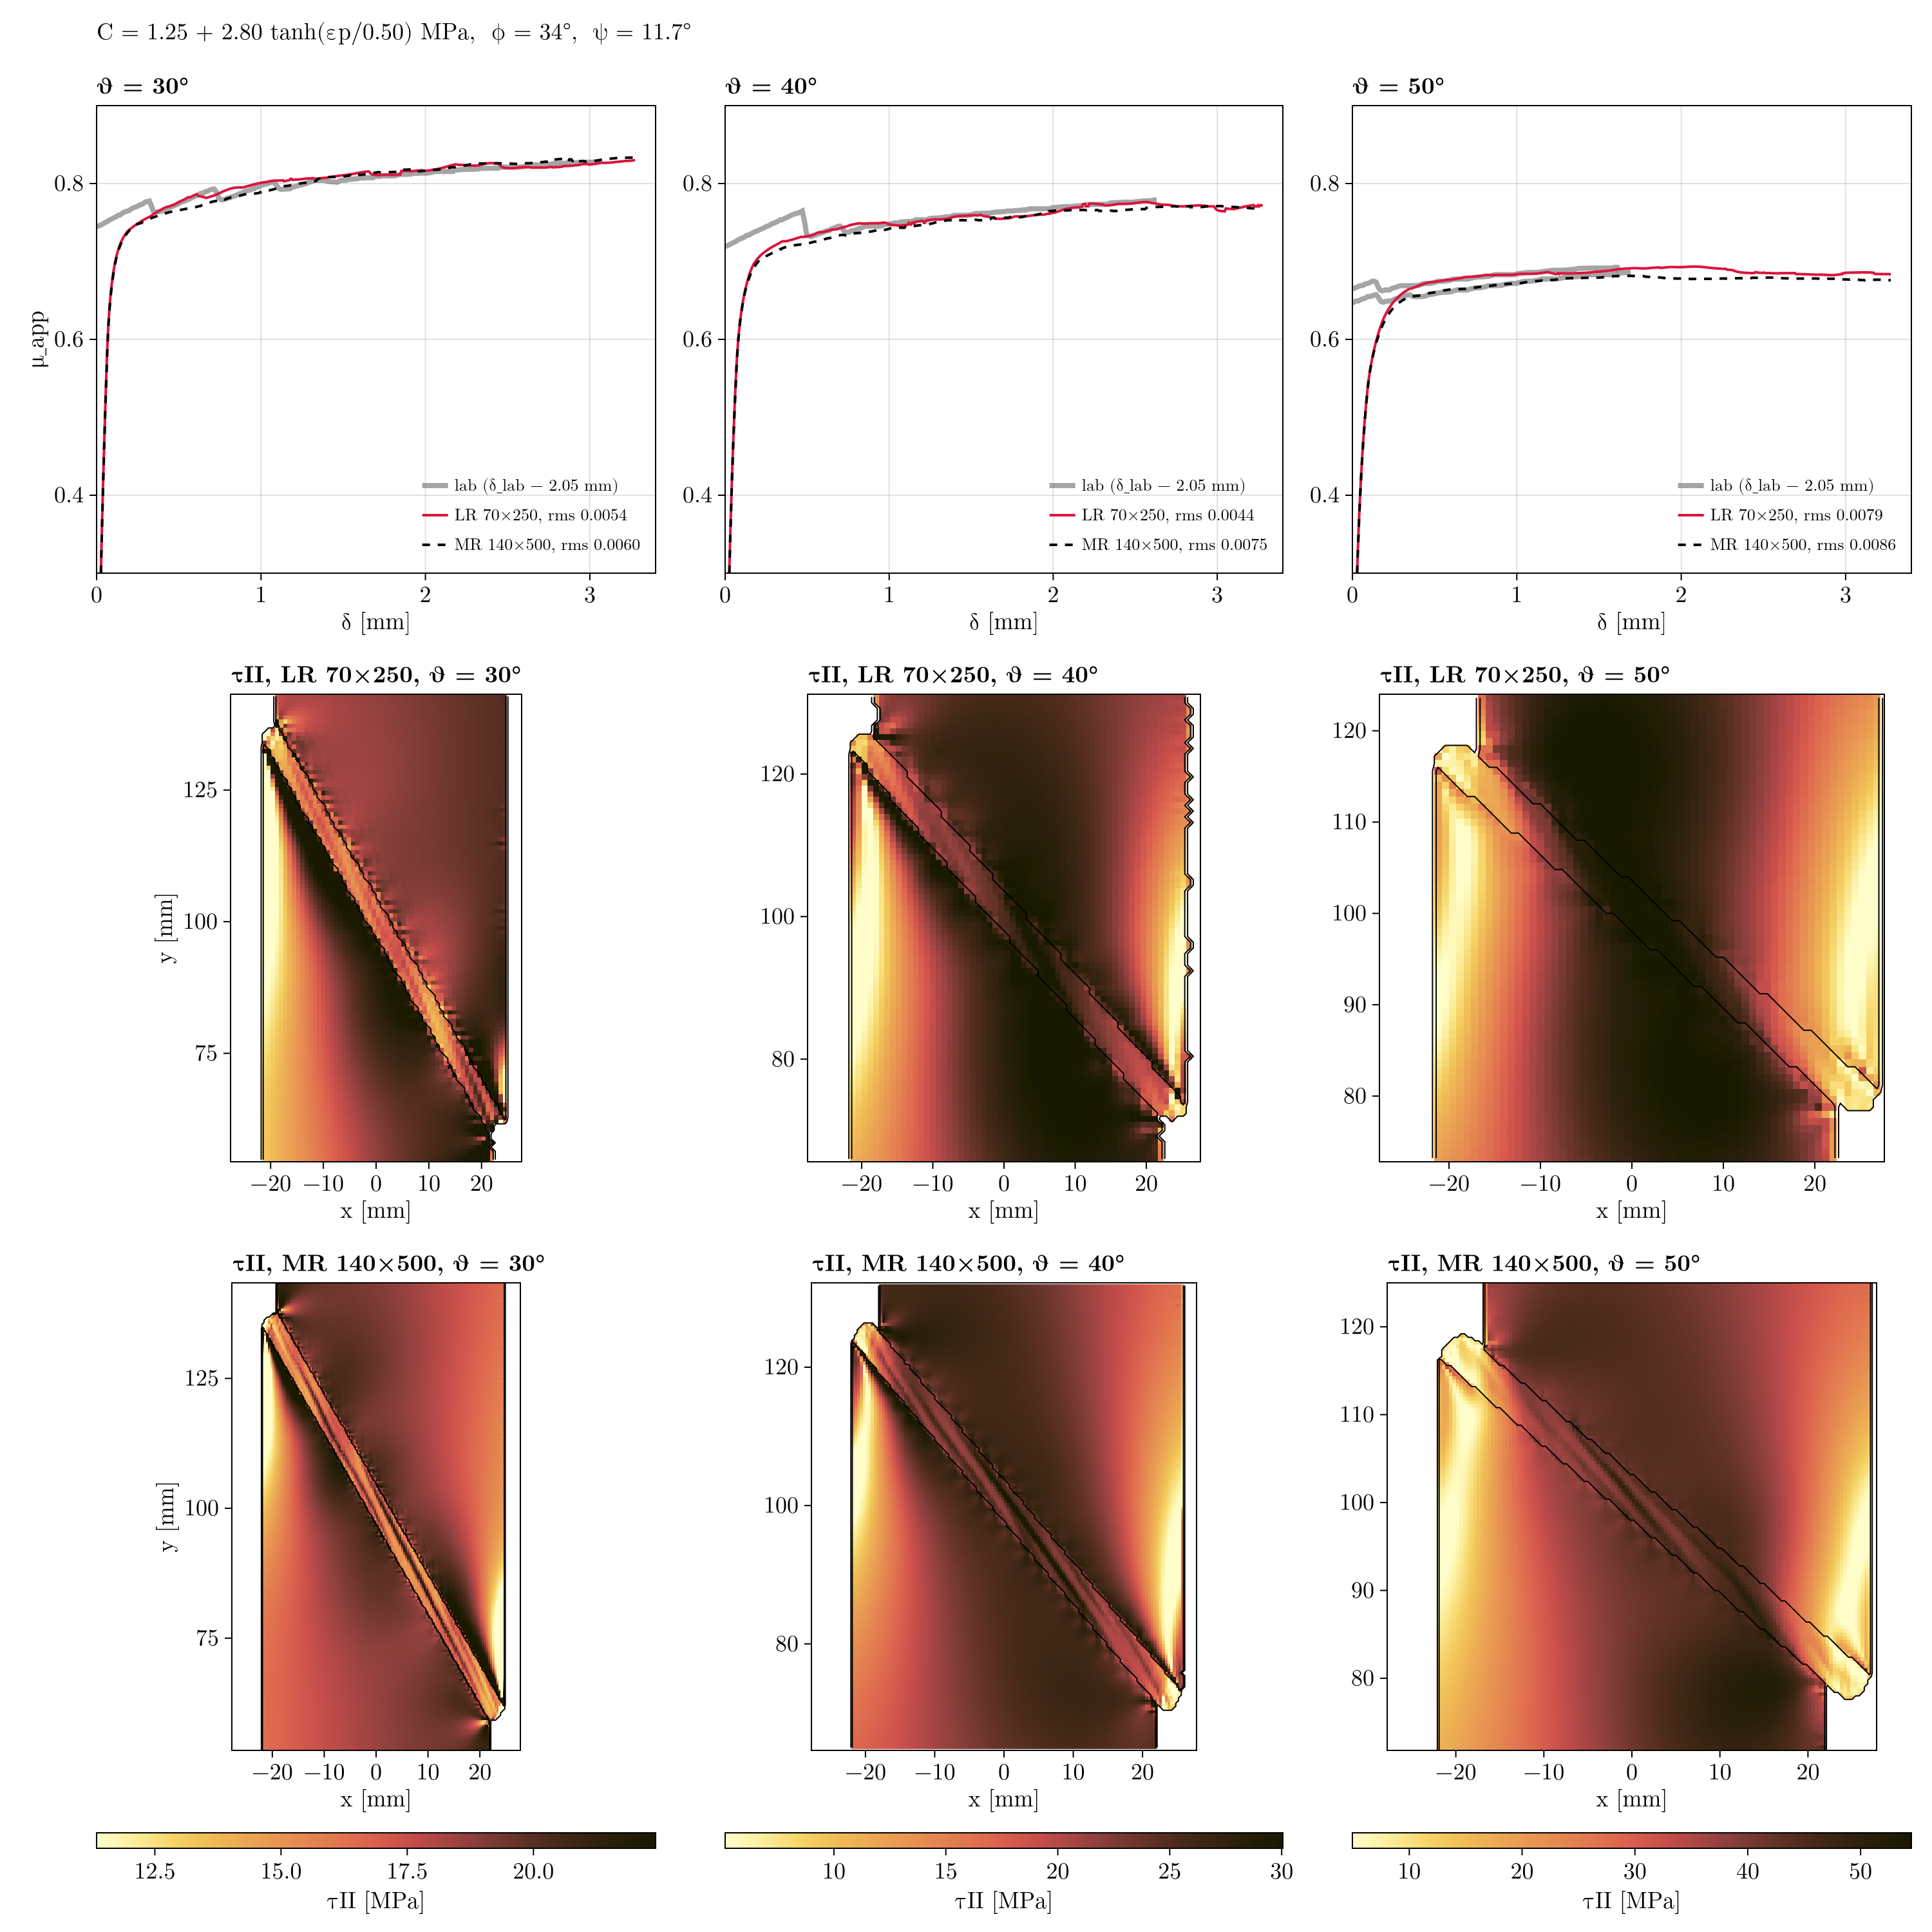
\includegraphics[width=0.92\textwidth]{figures/refit_resolution_C1.25_dC2.80_eh0.50_psi11.7.png}
\caption{Refit with scheme~1. Top: apparent friction at LR and MR against the lab curves, which are shifted by 2.05\,mm. Rows 2--3: $\tauII$ at the last step, LR and MR, with one colour range per angle.}\label{fig:res}
\end{figure}

\paragraph{Scheme comparison.} All seven schemes were run with the same parameters at MR, $\theta=40^\circ$, 6 threads, one run at a time (Table~\ref{tab:mr}, Figs.~\ref{fig:tau}--\ref{fig:cost}). Here ``rheology'' is the time spent in residual evaluation and line search, both of which call the constitutive update.

\begin{table}[h]\centering\small
\caption{MR, $\theta=40^\circ$, 12\,500\,s of loading in 500 steps. ``Failed'' counts time steps that were restarted with a smaller $\Delta t$.}\label{tab:mr}
\resizebox{\textwidth}{!}{\begin{tabular}{lrrrrrrr}
\toprule
scheme & $\mu_\mathrm{end}$ & rms vs.\ lab & Newton its & failed & wall [s] & rheology [s] & solve [s]\\
\midrule
0 legacy               & 0.762 & 0.0152 & 2134 & 0 & 1853 &  115 & 1458\\
1 iso-strain, grid     & 0.769 & 0.0075 & 1772 & 0 & 1863 &  167 & 1261\\
2 iso-strain, markers  & 0.773 & 0.0076 & 2156 & 0 & 2569 &  793 & 1498\\
3 iso-stress, grid     & 0.759 & 0.0181 & 1593 & 0 & 1567 &  133 & 1137\\
4 iso-stress, markers  & \multicolumn{7}{l}{stopped at step 119 ($\delta=0.33$\,mm) after 88\,min: 46 failed steps, 13.7 Newton its/step}\\
5 iso-work, grid       & 0.772 & 0.0064 & 1835 & 0 & 2009 &  272 & 1295\\
6 iso-work, markers    & 0.773 & 0.0099 & 2156 & 0 & 3996 & 2261 & 1496\\
\bottomrule
\end{tabular}}
\end{table}

\begin{figure}[p]\centering
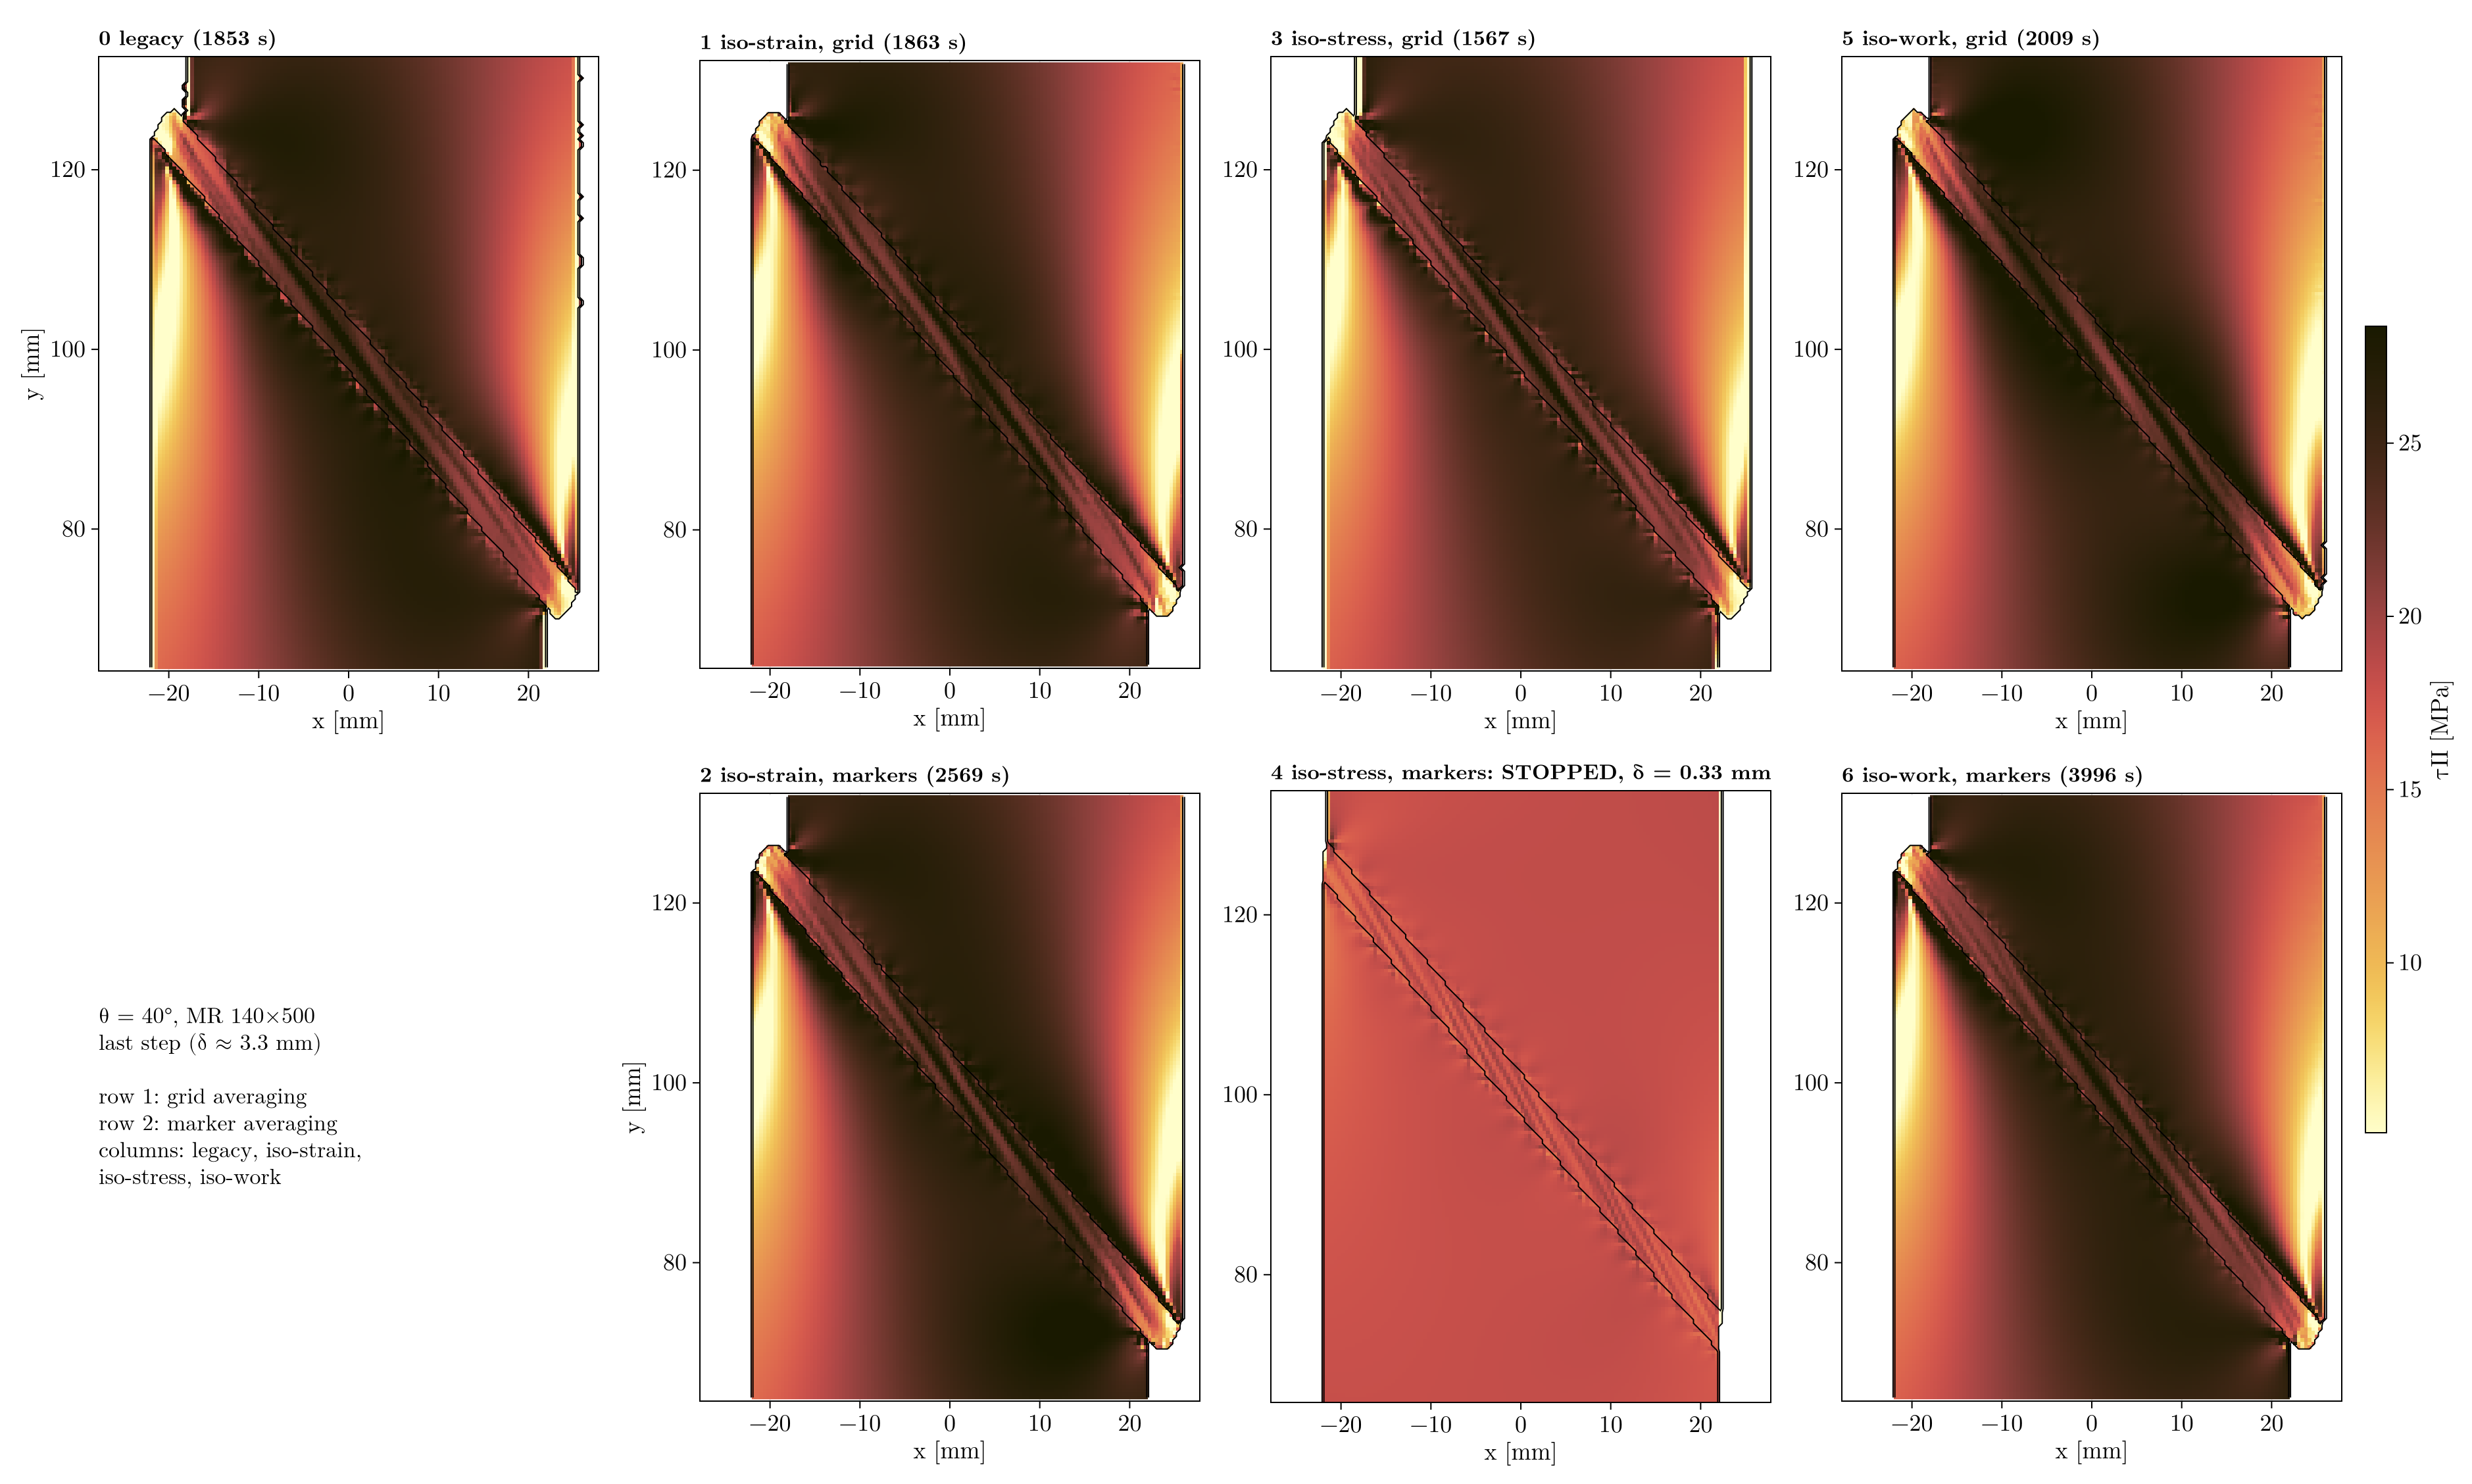
\includegraphics[width=\textwidth]{figures/schemes_MR_Tet40_tauII.png}
\caption{$\tauII$ at the last step (rock only), MR, $\theta=40^\circ$, common colour range. Row~1: grid averaging; row~2: marker averaging. Scheme~4 is shown at the step where it was stopped.}\label{fig:tau}
\vspace{4mm}
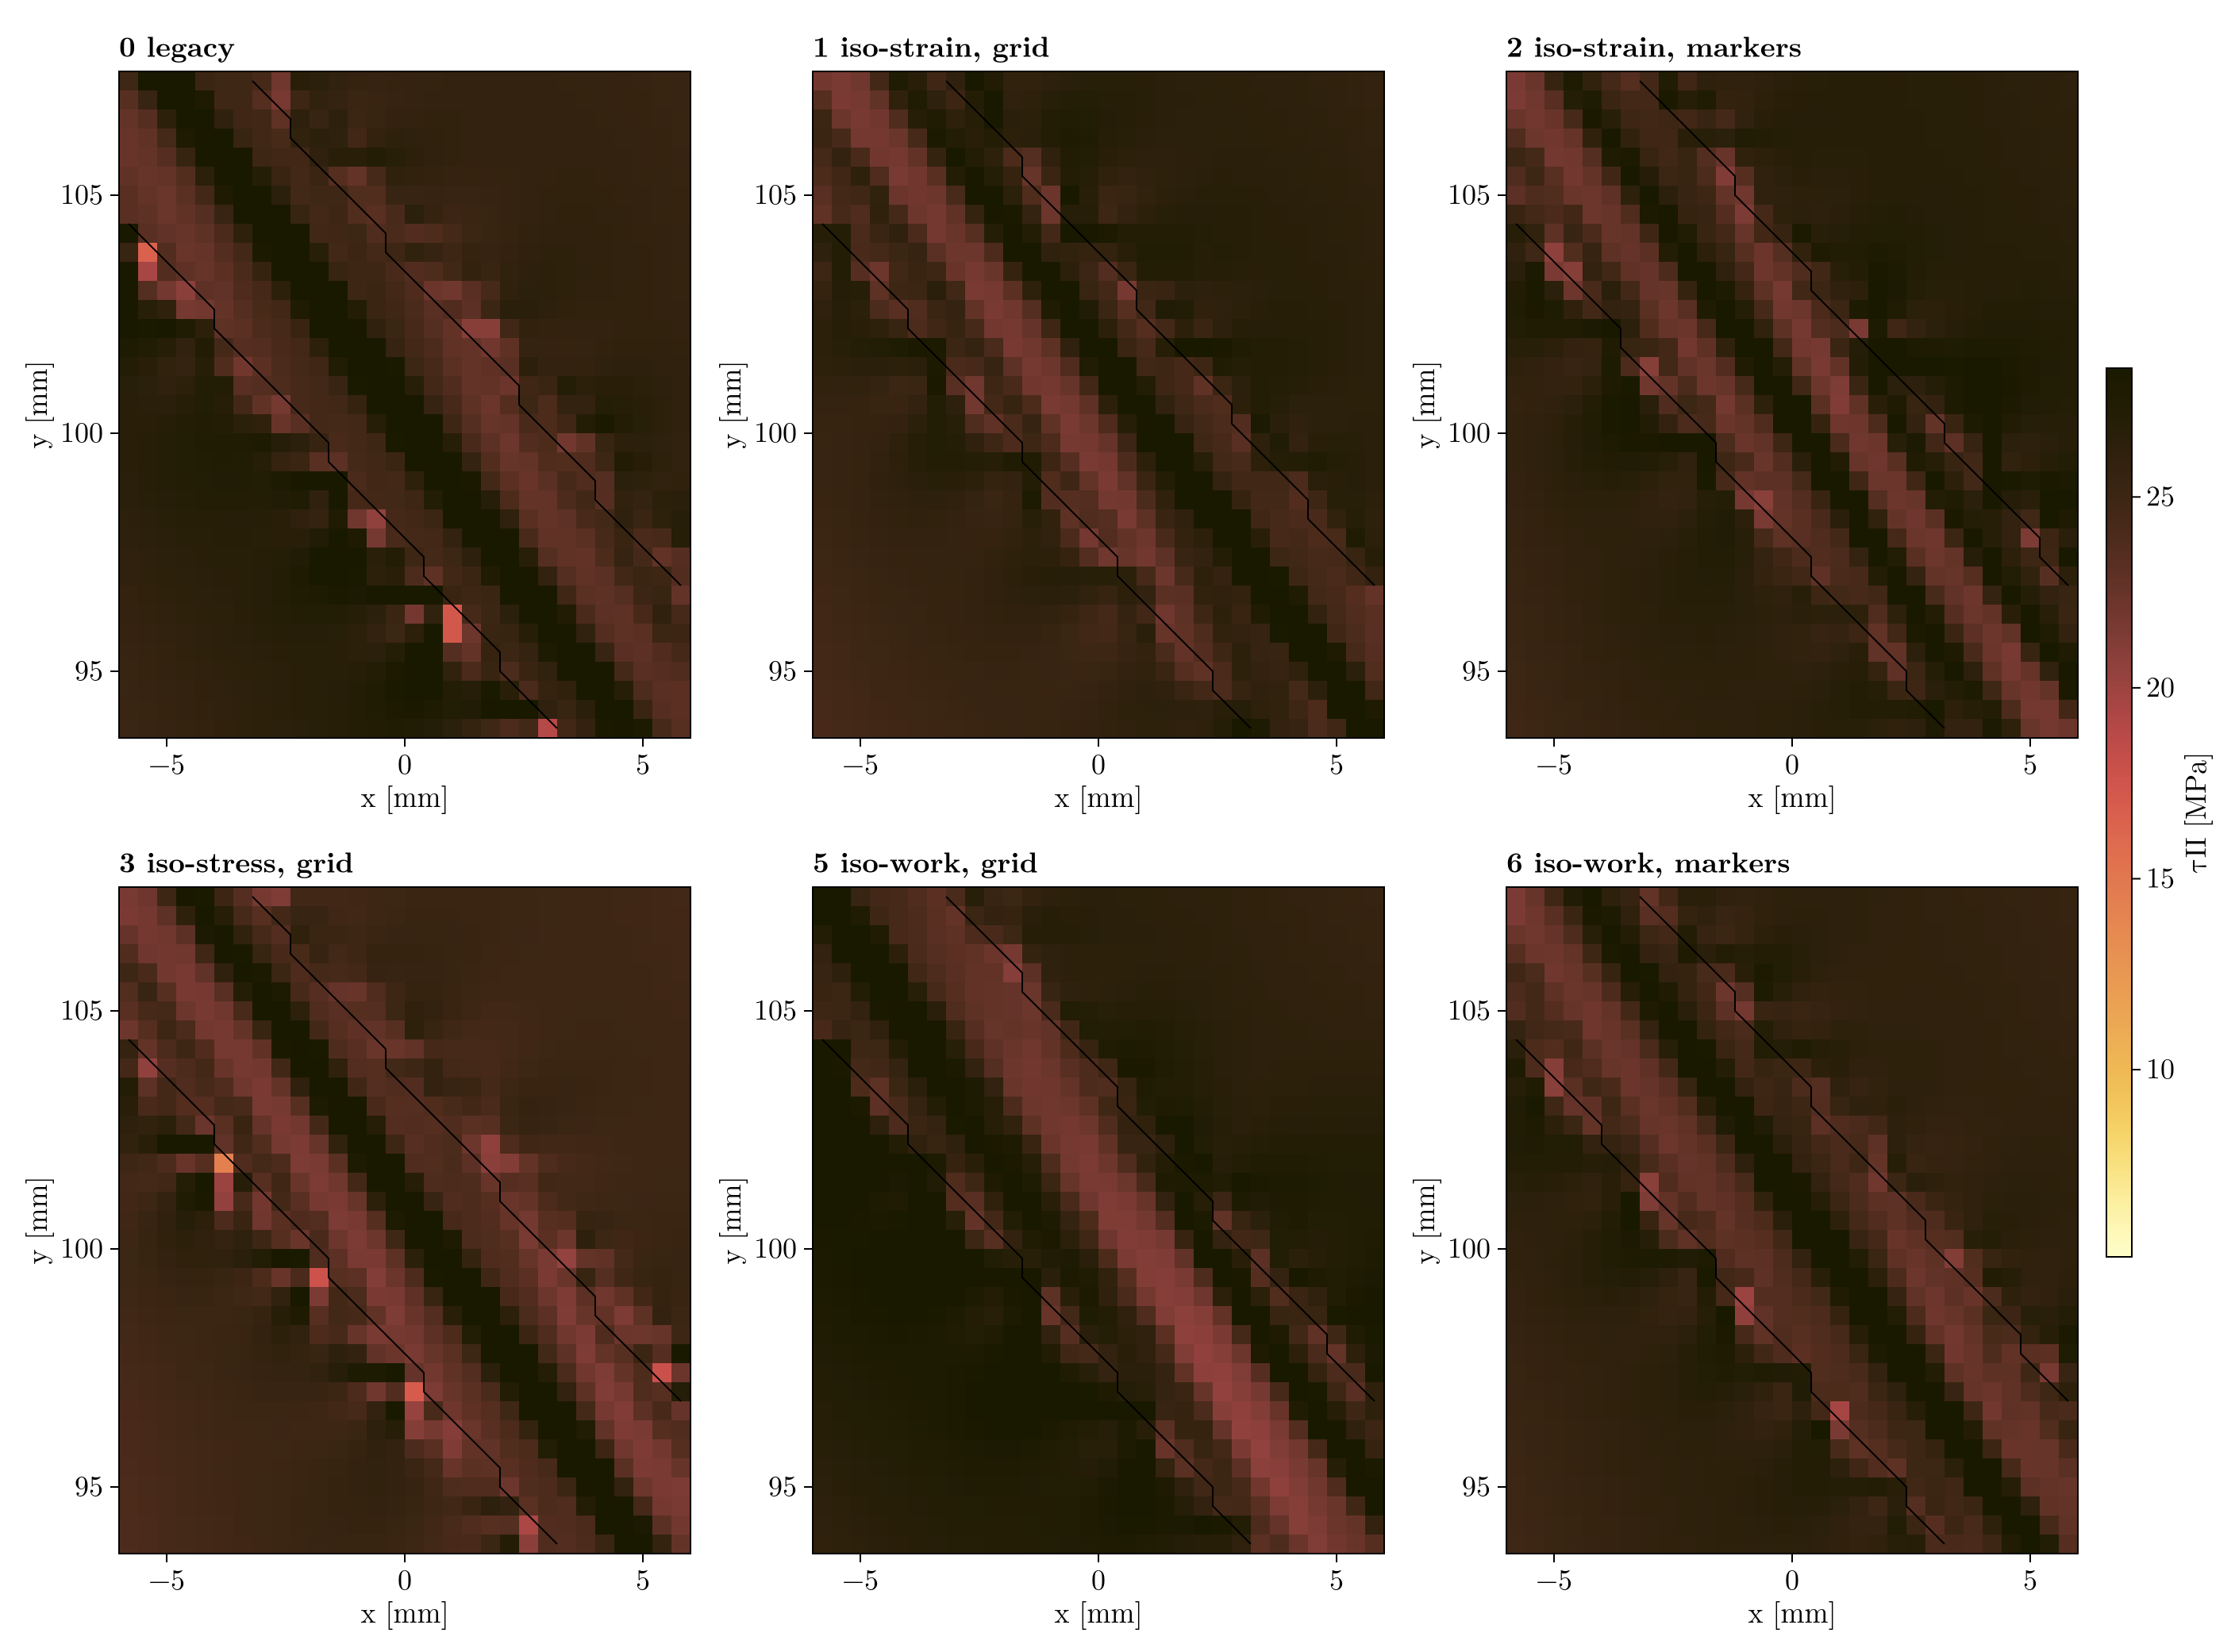
\includegraphics[width=0.85\textwidth]{figures/schemes_MR_Tet40_tauII_zoom.png}
\caption{Zoom on the centre of the gouge (black: gouge phase-fraction contour 0.5, a staircase on the Cartesian grid).}\label{fig:zoom}
\end{figure}

\begin{figure}[h]\centering
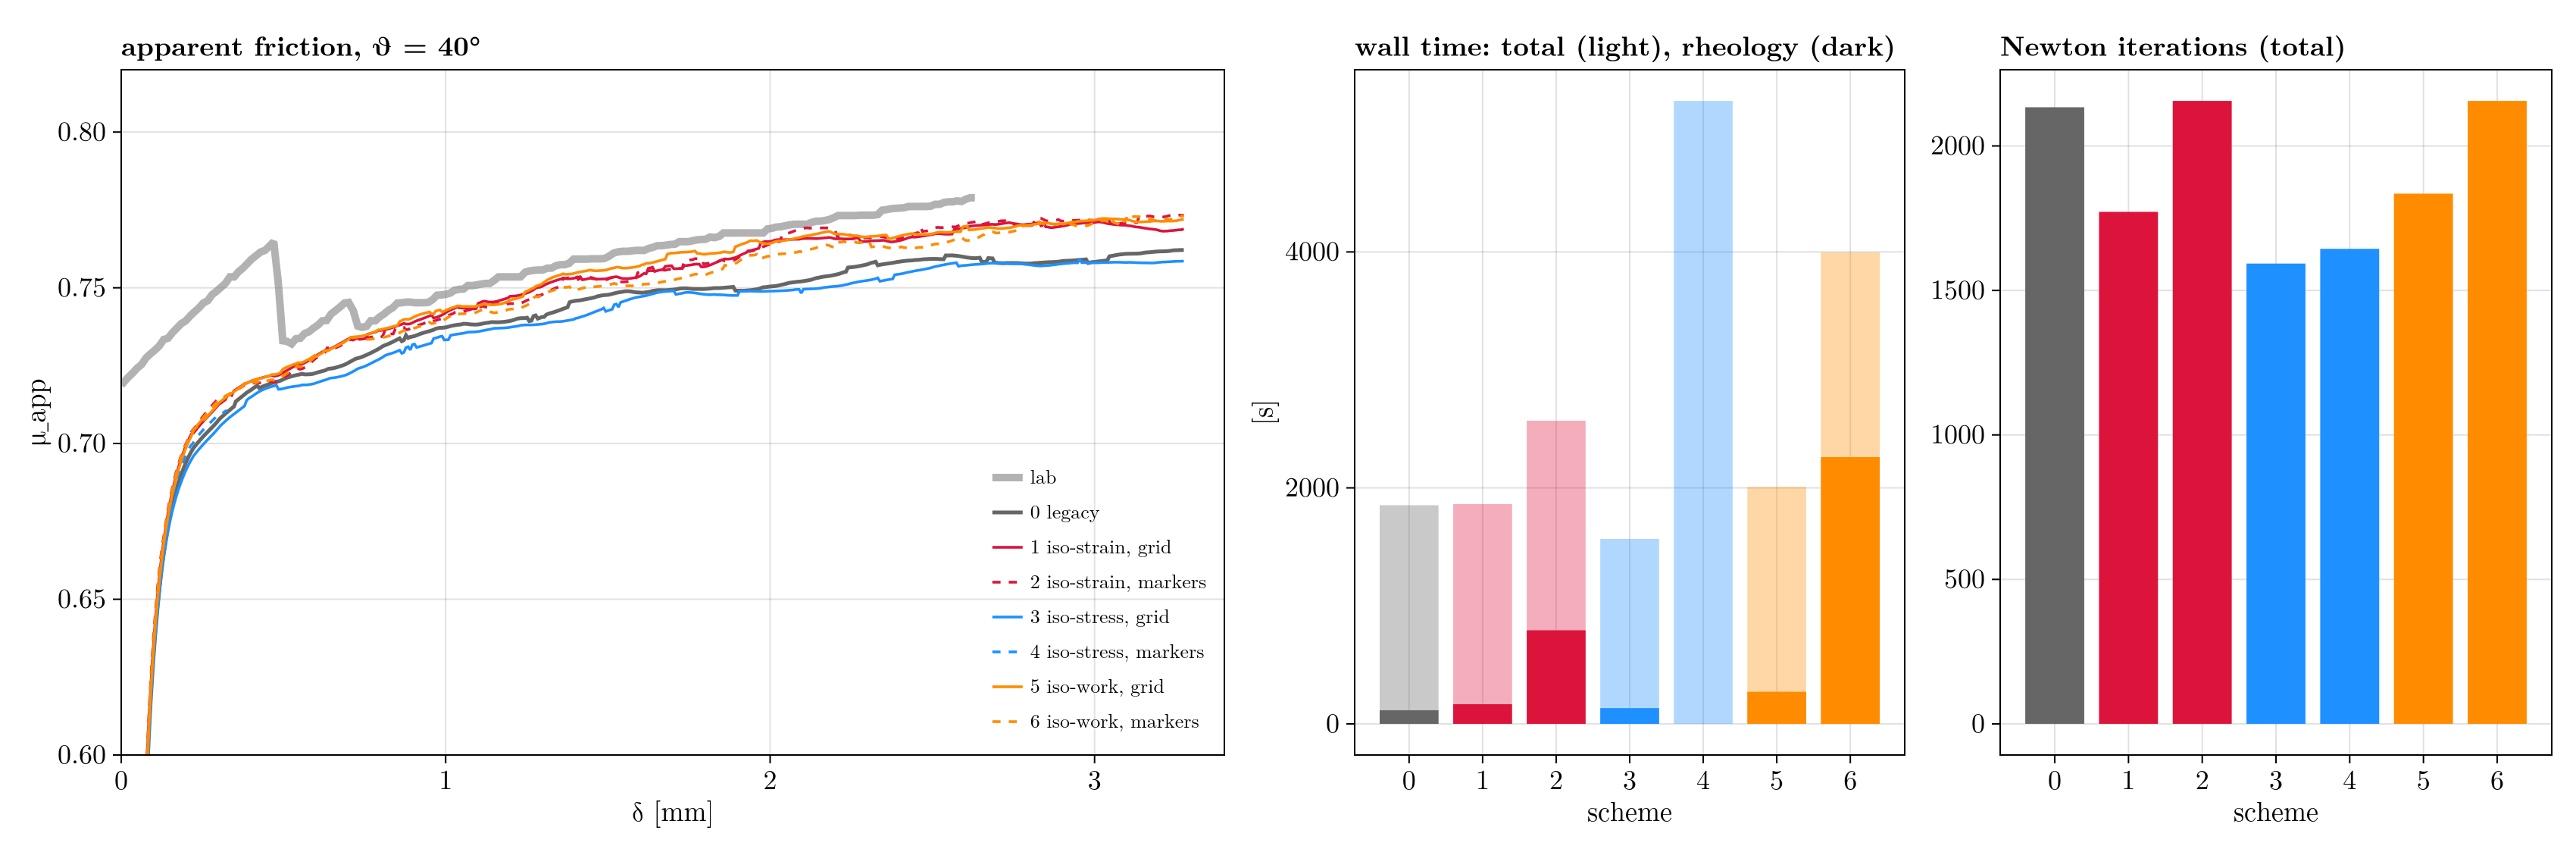
\includegraphics[width=\textwidth]{figures/schemes_MR_Tet40_friction_cost.png}
\caption{Left: apparent friction against the lab curve. Middle: wall time (light) and rheology time (dark). Right: total Newton iterations.}\label{fig:cost}
\end{figure}

\paragraph{Observations.}
\begin{itemize}
\item \textbf{Large-scale stress pattern.} It is the same for all converged schemes. The gouge is weaker than the rock, a load-bearing band runs through the rock along the lower boundary of the gouge, and there are low-stress shadows at the free corners. The odd look of the $40^\circ$ run therefore does not come from the averaging scheme.
\item \textbf{Interface staircase.} At $40^\circ$ the gouge boundary is a staircase of mixed cells. Schemes 0, 3, 2 and 6 show isolated cells of low stress at the staircase corners (Fig.~\ref{fig:zoom}); scheme~0 also shows horizontal streaks below the gouge. Schemes 1 and 5 (iso-strain and iso-work on the grid) are the smoothest.
\item \textbf{Friction.} The fit was made with scheme~1, so these differences show how sensitive the friction is to the scheme, not which scheme is better. Iso-strain and iso-work agree within 0.004. Iso-stress and legacy give 0.007--0.010 lower friction, which is about the spread between the two 50$^\circ$ lab tests.
\item \textbf{Cost.} The linear solve dominates (1100--1500\,s for every scheme). Grid rheology costs 115--270\,s; on markers it costs 4.8--8.3 times more (793\,s for iso-strain, 2261\,s for iso-work). As a result, scheme~2 is 1.4 times and scheme~6 2.1 times slower than scheme~1. Iso-stress on the grid is the cheapest (fewest Newton iterations) but has the worst friction and staircase artefacts.
\item \textbf{Scheme 4 fails.} It stalls at a residual of about $10^{-6}$ and Newton does not converge. The likely cause is an inner partition that is not converged tightly enough, which makes its tangent inconsistent. This was also seen at LR, where the run hit the step limit with 396 failed steps. It has not been diagnosed further.
\end{itemize}

\section{Viagra benchmark}

An elastic plate fixed at one end is bent by gravity, which is then switched off at $t_\mathrm{off}=9.9$\,kyr. The plate should recover its initial shape. The plate is stiff ($\eta^{ve}\approx G\Delta t\approx3\times10^{20}$\,Pa\,s) against a $10^{21}$\,Pa\,s matrix, at $51\times51$ resolution over 200 steps (Table~\ref{tab:viagra}, Fig.~\ref{fig:viagra}).

\begin{table}[h]\centering\small
\caption{Viagra test. Tip: mean $y$ of the plate markers with $x>750$\,km, minus 500\,km. Recovery: $1-\text{tip}_\mathrm{end}/\text{tip}_\mathrm{max}$. Edges: top and bottom plate edge offsets at the tip. Wall times are for warmed-up runs.}\label{tab:viagra}
\resizebox{\textwidth}{!}{\begin{tabular}{lrrrrrr}
\toprule
scheme & max tip [km] & final tip [km] & recovered & top edge [km] & bottom edge [km] & wall [s]\\
\midrule
0 legacy              & $-99.0$ & $-12.7$ & 87.2\% & $-13.0$ & $-8.2$ & 15\\
1 iso-strain, grid    & $-99.4$ & $-8.0$  & 92.0\% & $-17.6$ & $-8.4$ & 20\\
2 iso-strain, markers & $-99.0$ & $-7.8$  & 92.1\% & $-16.9$ & $-8.1$ & 22\\
3 iso-stress, grid    & $-99.0$ & $-9.5$  & 90.4\% & $-11.2$ & $-8.5$ & 13\\
4 iso-stress, markers & $-99.6$ & $-13.5$ & 86.5\% & $-10.0$ & $-8.8$ & 16\\
5 iso-work, grid      & $-99.3$ & $-9.7$  & 90.2\% & $-18.4$ & $-8.6$ & 20\\
6 iso-work, markers   & $-97.8$ & $-6.1$  & 93.8\% & $-17.2$ & $-8.4$ & 18\\
\bottomrule
\end{tabular}}
\end{table}

\begin{figure}[h]\centering
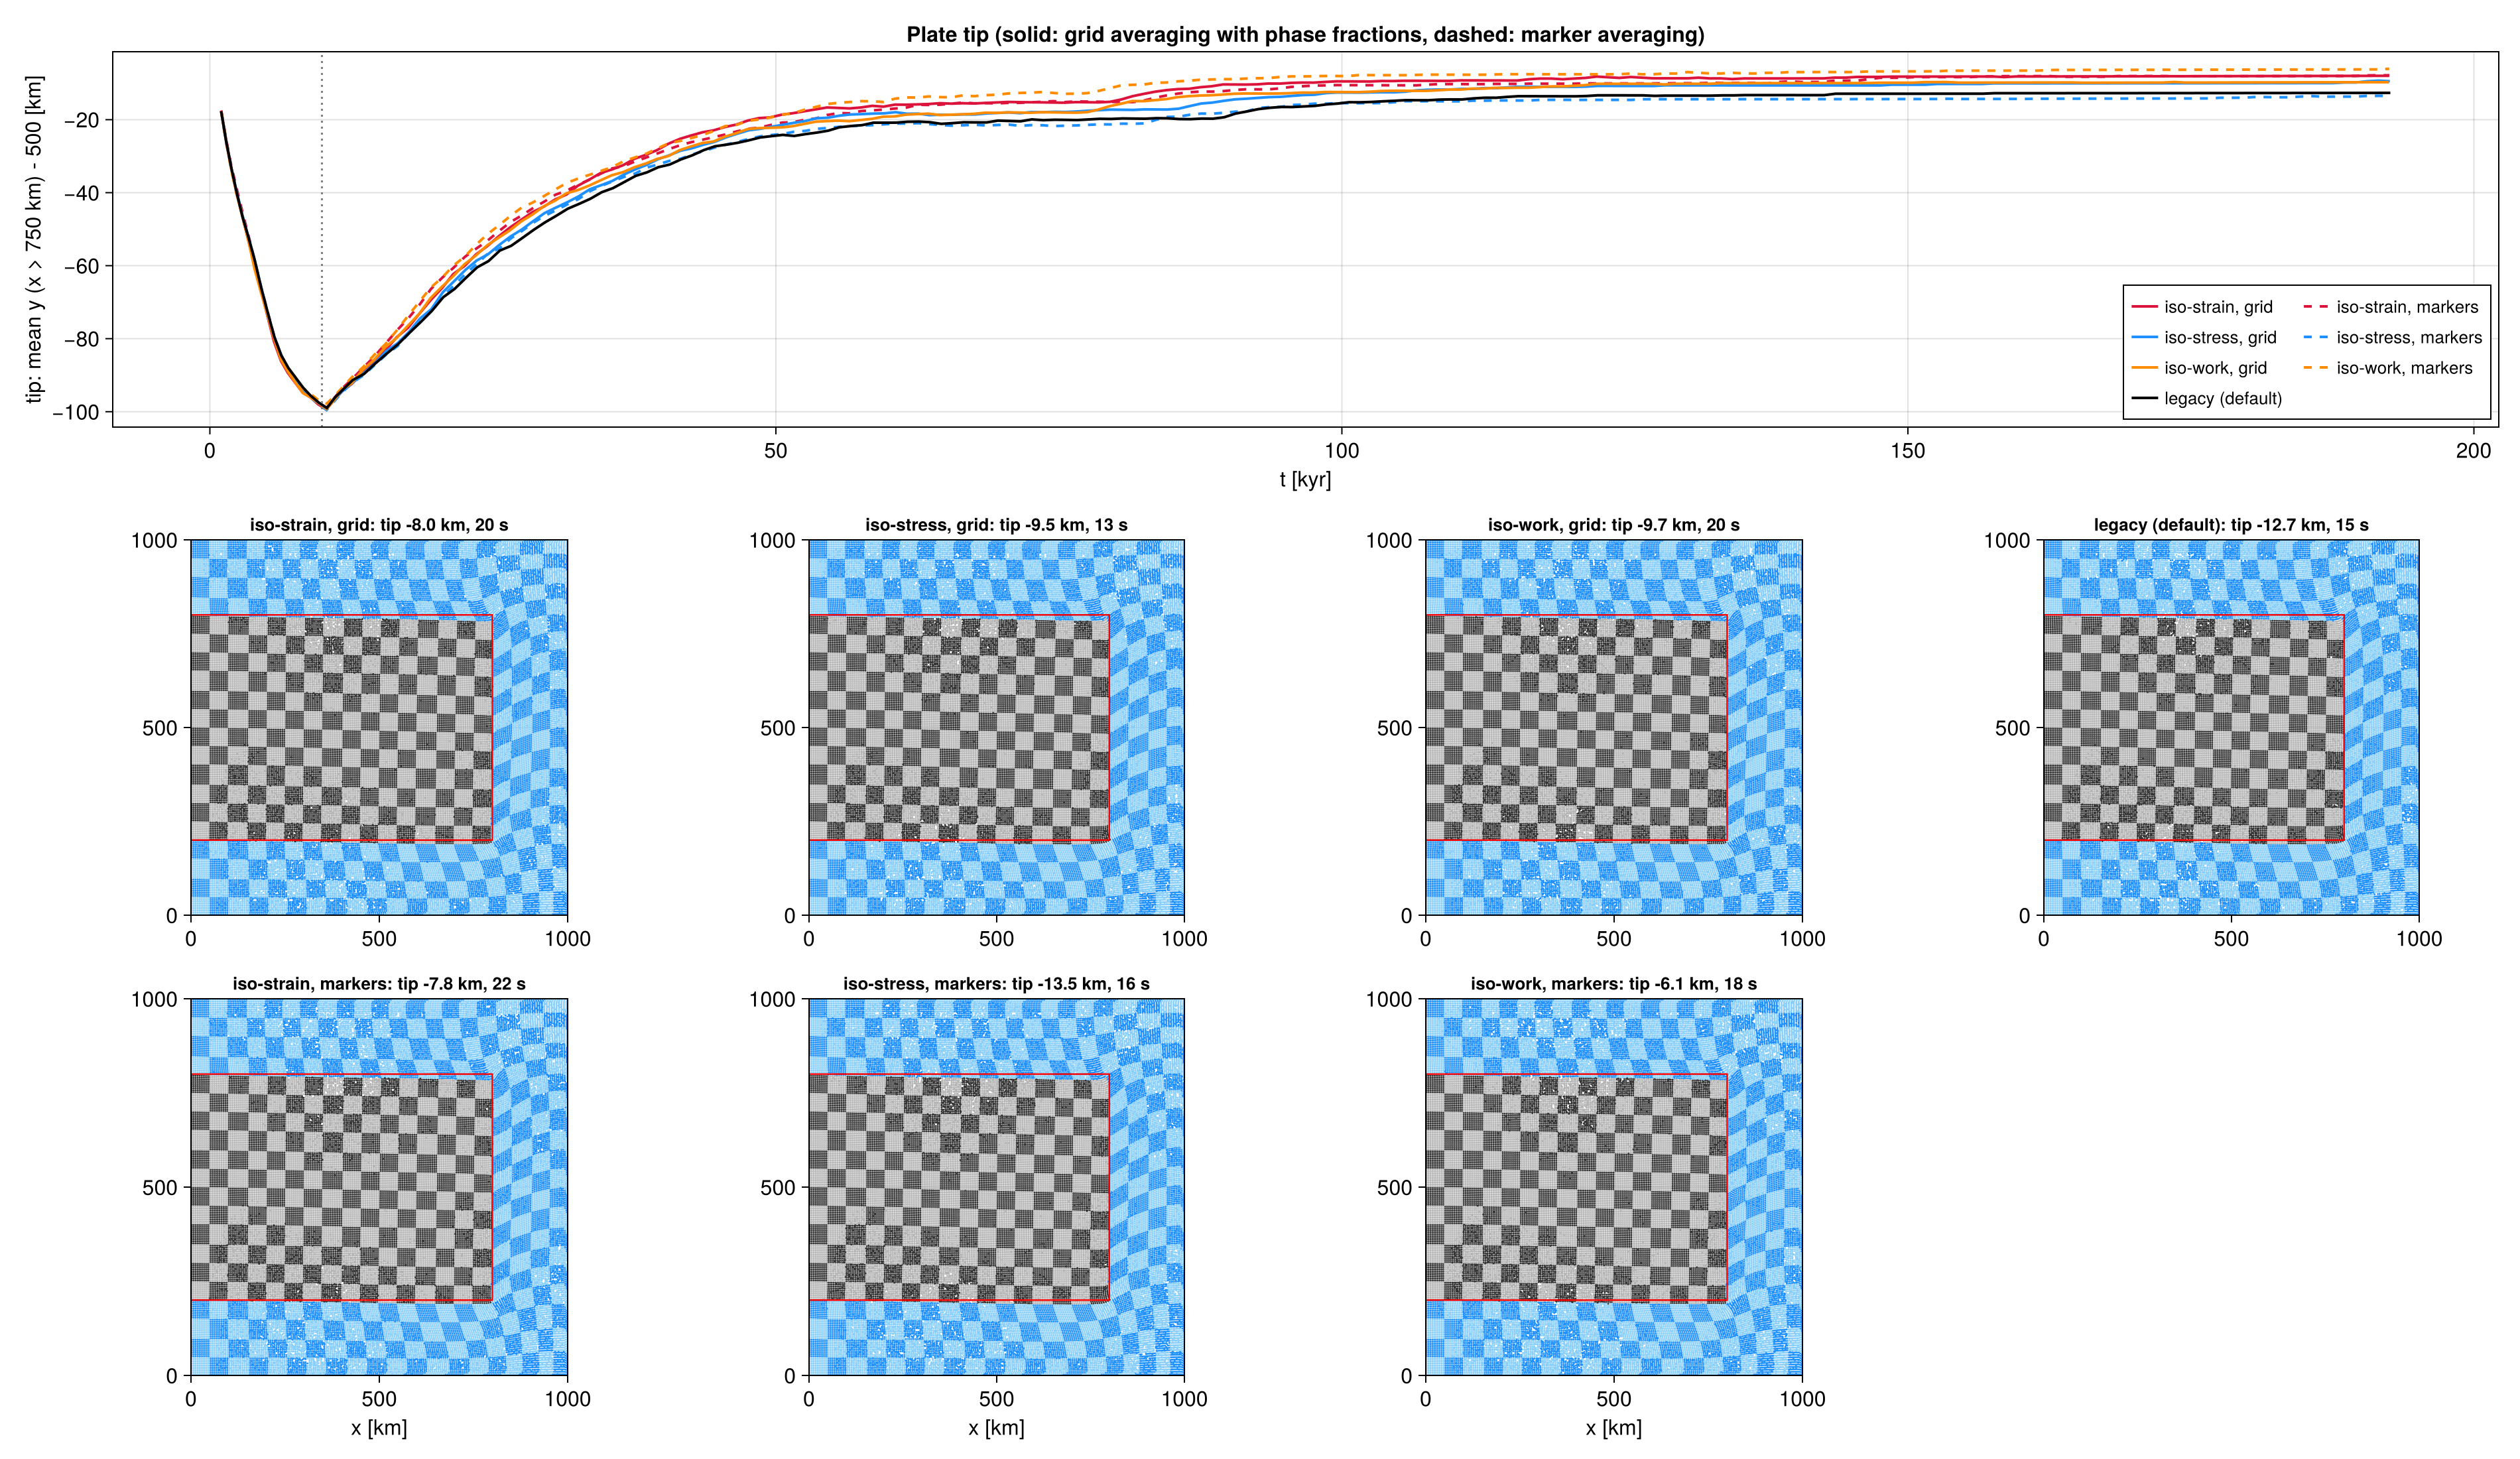
\includegraphics[width=\textwidth]{figures/ViagraMixing_grid_vs_markers_v3.png}
\caption{Viagra test. Top: plate tip deflection over time (dotted line: gravity switched off). Below: final marker positions.}\label{fig:viagra}
\end{figure}

\paragraph{Observations.} All schemes recover 86--94\% of the deflection. The ranking is iso-work/iso-strain > iso-stress > legacy, but the differences (6\,km) are small compared with the common residual offset of about 8\,km. That offset decreases with $\Delta t$ (first-order time error of the backward-Euler stress update together with frozen-velocity marker advection), so it is not caused by the averaging. Legacy and marker iso-stress recover least. The test discriminates weakly between schemes, because the plate's visco-elastic viscosity is only about 3 times lower than the matrix viscosity.

\section{Conclusions and choices}

\begin{enumerate}
\item \textbf{Default: iso-strain on the grid (scheme 1, \texttt{mixing=:voigt}, \texttt{plastic\_strain=:phase}).}
  \begin{itemize}
  \item It gives the cleanest stress at the staircase interfaces and the fewest Newton iterations among the accurate schemes.
  \item Its wall time is equal to legacy.
  \item It gives near-best Viagra recovery and is consistent with the lab fit.
  \end{itemize}
\item \textbf{Iso-work on the grid (scheme 5) is an equivalent alternative.} It gives the same friction and a similarly clean field, at 8\% more wall time and 1.6 times the rheology cost. It brings no clear benefit here.
\item \textbf{Marker averaging (2, 6) is not worth its cost} for these problems (1.4--2.1 times the wall time). It does not remove the staircase artefacts.
\item \textbf{Iso-stress} gives lower friction and artefacts on the grid, and fails on markers. Keep it for testing only.
\item \textbf{Legacy (0) should be retired.} It shows the strongest interface artefacts and the lowest Viagra recovery, and it evaluates each phase with the harmonic grid modulus.
\item \textbf{Fit:} $C=1.25+2.8\tanh(\eps_p/0.5)$\,MPa, $\phi=34^\circ$, $\psi=11.7^\circ$ with scheme~1. It holds at MR (rms $\le0.009$).
\end{enumerate}

\paragraph{Open items.}
\begin{itemize}
\item Marker iso-stress convergence (inner partition tolerance or tangent).
\item The about 8\,km Viagra offset is a time-discretisation error; a second-order scheme (BDF2) is postponed.
\item The staircase artefacts at oblique interfaces are common to all schemes and decrease with resolution.
\end{itemize}

\paragraph{Reproduce.}
\begin{itemize}
\item \texttt{ShearApparatus/\_hardening\_refit}: \texttt{queue\_schemes.sh}, \texttt{run\_fit.jl}, \texttt{plot\_schemes\_MR.jl}, \texttt{plot\_refit\_res.jl}.
\item \texttt{ViagraMixing}: \texttt{run\_viagra\_v3.jl}, \texttt{plot\_viagra\_v3.jl}.
\item \texttt{ShearApparatus/\_alloc\_test/alloc\_test.jl}.
\item \texttt{ShearApparatus/\_dilatancy\_test/dilatancy\_box.jl}.
\end{itemize}

\end{document}
